
 %%%%%%%%%%%%%%%%%%%%%%%%%%%%%%%%%%%%%%%%%%%%%%%%%%%%%%%%%
 %
 %	Name			:: 	The official template for the typesetting of diploma theses at the Faculty of Computer Science of AGH University of Krakow
 %	Author			:: 	Stanisław Polak (polak[aT]icsr[DoT]agh[DoT]edu[DoT]pl)
 %	Created			::	2024-02-14
 %	Modified	    ::	2024-03-04
 %	Version			:: 	1.3.1
 %	Email			:: 	polak[aT]icsr[DoT]agh[DoT]edu[DoT]pl
 %	Website			:: 	http://www.icsr.agh.edu.pl/~polak/
 %   Youtube         ::  https://www.youtube.com/user/spolak69
 %   Github          ::  https://github.com/polaksta
 %	License			:: 	This work may be distributed and/or modified under the
 %                       conditions of the LaTeX Project Public License, either version 1.3
 %                       of this license or (at your option) any later version.
 %                       The latest version of this license is in
 %                       http://www.latex-project.org/lppl.txt
 %                       and version 1.3 or later is part of all distributions of LaTeX
 %                       version 2005/12/01 or later.
 %
 %	Description		::	This document is a demonstration of the template
 %
 %%%%%%%%%%%%%%%%%%%%%%%%%%%%%%%%%%%%%%%%%%%%%%%%%%%%%%%%%
 % Niniejszy dokument — szkielet pracy dyplomowej — prezentuje przykłady użycia klasy 'agh-wi' oraz pakietów tradycyjnie używanych w pracach
 % dyplomowych z informatyki. Dla kilku z nich, wartości początkowe parametrów konfiguracyjnych są zdefiniowane 
 % w klasie  — wartości te uwzględniają uwagi osób prowadzących przedmiot "Pracownia Dyplomowa". 
 % Oczywiście możesz używać dowolnych pakietów, niekoniecznie tych, które są pokazane w tym dokumencie
 %%%%%%%%%%%%%%%%%%%%%%%%%%%%%%%%%%%%%%%%%%%%%%%%%%%%%%%%%
 % Poniższe uwagi NIE DOTYCZĄ Overleaf-a
 %%%%%%%%%%%%%%%%%%%%%%%%%%%%%%%%%%%%%%%%%%%%%%%%%%%%%%%%%
 % W tej przykładowej pracy dyplomowej użyto, między innymi, pakietów:
 %   - "minted", co oznacza, że musisz uruchomić kompilator z opcją '-shell-escape'
 %   - "biblatex", co oznacza, że po kompilacji (dokumentu) musisz, jeszcze, wygenerować plik '.bbl'
 %   - "nomencl", co oznacza, że za pomocą komendy 'makeindex' musisz wygenerować wykaz symboli
 %
 % Tak więc, w celu wygenerowania wynikowego dokumentu PDF, musisz wykonać następujące komendy:
 %       pdflatex -shell-escape example
 %       biber example
 %       makeindex example.nlo  -s nomencl.ist -o example.nls
 %       pdflatex -shell-escape example
 %       pdflatex -shell-escape example
 %
 % Dodatkowo musisz mieć zainstalowany program 'pygmentize', który jest częścią pakietu "Pygments" (https://pygments.org/)
 % Ww. programy powinny zainstalować się automatycznie podczas instalacji pakietów LaTeX
 %
 % Jeżeli masz zainstalowany program 'latexmk', to możesz wygenerować dokument PDF następująco:
 %       latexmk example
 %       makeindex example.nlo  -s nomencl.ist -o example.nls
 %       latexmk example
 %
 % Do edycji (oraz komplilacji) dokumentów LaTeX polecam program 'TeXstudio' (https://www.texstudio.org/)
 %
 % Autor: Stanisław Polak <polak[aT]agh[DoT]edu[DoT]pl>
 %%%%%%%%%%%%%%%%%%%%%%%%%%%%%%%%%%%%%%%%%%%%%%%%%%%%%%%%%
 \documentclass[english, print]{agh-wi} % Praca po polsku; na stronie tytułowej, najpierw jest widoczny polskojęzyczny tytuł, a potem angielskojęzyczny.
 % Kierunek 'Informatyka'.
 % Przeznaczona do oglądania przy użyciu przeglądarki PDF.
%%%%%%%%%%%%%%%%%%%%%%%%%%%%%%%%%
% Inne, przykładowe, użycia klasy
%%%%%%%%%%%%%%%%%%%%%%%%%%%%%%%%%
% \documentclass[english]{agh-wi}               % Praca po angielsku; 
						   %     strona tytułowa po polsku, ale najpierw jest widoczny angielskojęzyczny tytuł, a potem polskojęzyczny.  
						   % Kierunek 'Informatyka'.
						   % Przeznaczona do oglądania przy użyciu przeglądarki PDF.
% \documentclass[english, data-science]{agh-wi} % Praca po angielsku; ...
						   % Kierunek 'Informatyka - Data Science'.
						   % Przeznaczona do oglądania przy użyciu przeglądarki PDF.
% \documentclass[print]{agh-wi}                 % Praca po polsku; ...
						   % Kierunek 'Informatyka'.
						   % Przeznaczona do drukowania - każda strona posiada,
						   %    dodatkowy (2cm), margines na oprawę.
%%%%%%%%%%%%%%%%%%%%%%%%%%%%%%%%%%%%%
% Parametry dla strony tytułowej
%%%%%%%%%%%%%%%%%%%%%%%%%%%%%%%%%%%%%
\titlePL{Globalna lokalizacja agenta w oparciu o segmenty płaszczyzn}  % Tytuł po polsku
\titleEN{Planar segment-based global localization for autonomous agents} % Tytuł po angielsku
\author{Jan Rodzoń}
\supervisor{prof dr hab. inż. Bogdan Kwolek}
%%%%%%%%%%%%%%%%%%%%%%%%%%%%%%%%%%%%%
% Pakiety
%%%%%%%%%%%%%%%%%%%%%%%%%%%%%%%%%%%%%
% Podstawowe — na pewno będziesz ich potrzebował(a) w swojej wersji pracy dyplomowej
%%%%%%%%%%%%%%%%%%%%%%%%%%%%%%%%%%%%%
\usepackage{polski} % Obsługa języka polskiego
%%% fix for \lll
\let\babellll\lll
\let\lll\relax
%%%%%%%%%%%%%%%%%%%%%%%%%%%%%%%%%%%%%
% Dodatkowe — niekoniecznie będziesz ich potrzebował(a) w swojej wersji pracy dyplomowej
%%%%%%%%%%%%%%%%%%%%%%%%%%%%%%%%%%%%%			
\usepackage[sorting=none]{biblatex}           % Spis literatury ma być tworzony na podstawie zawartości bibliograficznej bazy danych
\usepackage{amsmath}                          % Dodatkowe środowiska matematyczne
\usepackage{amssymb}                          % Dodatkowe symbole matematyczne
%%% fix for \lll
\let\mathlll\lll
\let\lll\babellll
\usepackage[polish, intoc]{nomencl}           % Definiowanie symboli
\usepackage{graphicx}                         % Wstawianie grafik zewnętrznych
\usepackage{xcolor}                           % Kolorowy tekst
\usepackage{colortbl}                         % Kolory w tabeli
\usepackage{tabularx}                         % Rozszerzona wersja środowiska 'tabular'
\usepackage{longtable}                        % Skład "długich" tabel
\usepackage[ruled,linesnumbered]{algorithm2e} % Algorytmy w formie pseudokodu
\usepackage{listings}                         % Formatowanie kodów źródłowych programów
\usepackage[newfloat]{minted}                 % Formatowanie kodów źródłowych programów
\usepackage{hyperref}                         % Obsługa adresów URL — zbędny jeżeli używasz 'biblatex'
\usepackage{csquotes}                         % Polskie cudzysłowy — rekomendowany jeżeli używasz 'biblatex'
\usepackage{float}

% My additional packages
\usepackage{blindtext}
%%%%%%%%%%%%%%%%%%%%%%%%%%%%%%%%%%%%
%  % Konfiguracja rysunków TikZ
%%%%%%%%%%%%%%%%%%%%%%%%%%%%%%%%%%%%
\usetikzlibrary{shapes.geometric,arrows.meta} 
\tikzstyle{every picture}+=[remember picture]
\tikzstyle{na} = [baseline=-.5ex]
%%%%%%%%%%%%%%%%%%%%%%%%%%%%%%%%%%%%
% Ładowanie danych bibliograficznych
%%%%%%%%%%%%%%%%%%%%%%%%%%%%%%%%%%%%
\addbibresource{bibliography.bib}
%%%%%%%%%%%%%%%%%%%%%%%%%%%%%%%%%%%%%
% Opcje konfiguracyjne pakietów
%%%%%%%%%%%%%%%%%%%%%%%%%%%%%%%%%%%%%
% Pakiet 'framed'
\definecolor{shadecolor}{gray}{0.9}
% Pakiet 'nomencl'
\makenomenclature % Otwórz plik 'example.nlo'
%%%%%%%%%%%%%%%%%%%%%%%%%%%%%%%%%%%%%
% Definicje komend
%%%%%%%%%%%%%%%%%%%%%%%%%%%%%%%%%%%%%
\newcommand{\alert}[1]{\colorbox{red!50}{#1}}
\newcommand{\bt}{\blindtext}
\newcommand{\rev}[1]{#1}
\newcommand{\T}[1]{\texttt{#1}}
\newcommand\todo[1]{\textcolor{red}{#1}}
%%%%%%%%%%%%%%%%%%%%%%%%%%%%%%%%%%%%%
% Twierdzenia i podobne struktury
%%%%%%%%%%%%%%%%%%%%%%%%%%%%%%%%%%%%%
\newtheorem{theorem}{Twierdzenie}
\newtheorem{definition}{Definicja}

\newcounter{comment}[chapter]
\newenvironment{comment}[1][]{\begin{shaded}\refstepcounter{comment}
\noindent \textbf{Uwaga~\thechapter.\thecomment. #1} \rmfamily}{\end{shaded}}
%%%%%%%%%%%%%%%%%%%%%%%%%%%%%%%%%%%%%
% Treść poszczególnych rozdziałów tej, przykładowej, pracy dyplomowej 
%   znajduje się w osobnych plikach (patrz  katalog 'tex') 
%   i jest dołączana, do bieżącego pliku, komendą \include. 
% Tworząc pracę, z reguły, zajmujesz się edycją 
%   tylko jednego rozdziału. 
% Aby skrócić czas kompilacji warto, za pomocą komendy \includeonly, 
%   włączyć kompilację tylko tego pliku (rozdziału) nad którym, aktualnie, pracujesz
%%%%%%%%%%%%%%%%%%%%%%%%%%%%%%%%%%%%%
% \includeonly{tex/example,tex/notes} % Kompiluj, tylko, treść wymienionych plików, tj. 'tex/example.tex' oraz 'tex/notes.tex'.
%%%%%%%%%%%%%%%%%%%%%%%%%%%%%%%%%%%%%
%%%%%%%%%%%%%%%%%%%%%%%%%%%%%%%%%%%%%
\begin{document}
%%%%%%%%%%%%%%%%%%%%%%%%%%%%%%%%%%%%%
\frontmatter % Część wstępna
%%%%%%%%%%%%%%%%%%%%%%%%%%%%%%%%%%%%%
\maketitle % Dodaj stronę tytułową
%%%%%%%%%%%%%%%%%%%%%%%
% Jeżeli chcesz komuś podziękować, to możesz użyć poniższego kodu
\cleardoublepage
\thispagestyle{empty}
\vspace*{\fill}
\begin{flushright}
    \em
    \begin{minipage}{0.75\textwidth}
        Składam szczególne podziękowania mojemu Promotorowi, prof. dr hab. inż. Bogdanowi Kwolek
		za życzliwość, wszechstronne wsparcie, cierpliwość, cenne uwagi merytoryczne oraz poświęcony czas.
    \end{minipage}
\end{flushright}
%%%%%%%%%%%%%%%%%%%%%%%
\begin{abstractPL}
Niniejsza praca bada obecne rozwiązania i architektury sieci neuronowych
pod kątem lokalizacji agenta w oparciu o rozpoznawanie segmentów płaszczyzn na zdjęciach RGB.
W ramach pracy wybrano oraz sprawdzono zastosowanie kilku najnowszych technologii
opartych o sieci neuronowe w radzeniu sobie z rozpoznawaniem segmentów płaszczyzn
w różnych warunkach życia codziennego.
\end{abstractPL}
\begin{abstractEN}
This thesis examines current neural network solutions and architectures
in terms of agent localization based on recognition of plane segments from RGB images.
The work selects and tests the application of several state-of-the-art technologies
based on neural networks in dealing with the recognition of plane segments
in various everyday conditions.
\end{abstractEN}
%%%%%%%%%%%%%%%%%%%%%%%%%%%%%%%%%%%%%
%%%%%%%%%%%%%%%%%%%%%%%%%%%%%%%%%%%%%
\tableofcontents   % Wygeneruj spis treści
\listoffigures     % Wygeneruj listę rysunków
\listoftables      % Wygeneruj listę tabel
% Wygeneruj listę kodów źródłowych
\lstlistoflistings % Jeżeli do tworzenia listingów używasz pakietu 'listings'
%  \listoflistings % Jeżeli do tworzenia listingów używasz pakietu 'minted'i

%%%%%%%%%%%%%%%%%%%%%%%%%%%%%%%%%%%%%
\mainmatter % Część główna
%%%%%%%%%%%%%%%%%%%%%%%%%%%%%%%%%%%%%
% Rozdziały części głównej

\chapter{Preface}

We live in the era of automation.
Everywhere robots are taking over the positions, which require not only repetitive actions but also more complicated tasks.
In this environment, there are more and more machines that are operating within some contained spaces like commercial buildings or warehouses.
There is also a growing market for indoor drone usage.
Because of that, there is a need for a means of autonomous localization of these machines, which we will call generically agents in this work.
Recent advances in computer vision and artificial intelligence come in handy and provide some models for localization based on planar segments.

\section{Motivation}

Unfortunately, when one tries to use or apply the latest state-of-the-art models and algorithms there are a lot of obstacles to it—starting from
missing environment requirements, through outdated libraries, which have dropped backward compatibility,
and finishing on overfitted models, which are good only within specific circumstances and are not applicable in ordinary indoor applications.
This thesis aims to contribute to the field of agent localization and plane segmentation
by reviewing the current development of plane segmentation and measuring its potential on data
that is completely different from the training or testing one.
Additionally, some of the latest models are difficult to get started.
In this work, I also try to ease the workload required to get these projects going for future contributors or researchers.

\section{Content of this work}

The content of the chapters in this thesis is organized as follows:

\begin{enumerate}
\item \textbf{Chapter 2: Plane Segmentation Development} \ref{chap:plane-segmentation-development}

This chapter goes through the recent development in plane segmentation.
It compares different approaches and techniques to tackle this problem bringing up relevant literature.

\item \textbf{Chapter 3: Problem Description} \ref{chap:problem-description}

This chapter explains the problem of agent localization and the difficulties in applying it in everyday use.
It also covers the obstacles of running the latest state-of-the-art projects to deepen the research in this matter.

\item \textbf{Chapter 4: Implementation} \label{chap:implementation}

This chapter shows the actions taken to get the related projects up and running and to evaluate their usefulness in indoor applications,
including data preparation and processing.

\item \textbf{Chapter 5: Results Evaluation} \label{chap:results-evaluation}

This chapter presents and compares the results of the selected models.
It also shows how to get the related projects going after the contribution.

\item \textbf{Chapter 6: Conclusions} \ref{chap:conclusions}

This chapter concludes the results and shows potential directions for future work.

\end{enumerate}


\chapter{Problem formulation} \label{chap:problem-formulation}

Describe what each section contains...

\section{Issues to be addressed in this work}

\subsection{(e.g.) Algorithmic challenges}

\bt

\subsection{(e.g.) Parallelization challenges}

\bt

\section{Functional requirements}

\begin{enumerate}
	\item Core functionalities
	\begin{enumerate}
		\item ...
		\item ...
		\item ...
	\end{enumerate}

	\item Adaptation strategies
	\begin{enumerate}
		\item ...
		\item ...
	\end{enumerate}

	\item Visualization and profiling
	\begin{enumerate}
		\item ...
		\item ...
		\item ...
		\item ...
	\end{enumerate}
\end{enumerate}


\section{Non-functional requirements}

\begin{enumerate}
	\item Performance and complexity
	\begin{enumerate}
		\item ...
		\item ...
		\item ...
	\end{enumerate}

	\item Development requirements
	\begin{enumerate}
		\item ...
		\item ...
	\end{enumerate}
\end{enumerate}




\chapter{Solution methodology} \label{chap:methodology}

\bt

\section{Method 1}

\bt

\section{Method 2}

\bt 

\section{Method 3}

Some nice matrices...

\begin{equation}
	A = \begin{bmatrix}
		1 &    &    &    &    &    &    & \\
		1 & -2 &  1 &    &    &    &    & \\
		  &  1 & -2 &  1 &    &    &    & \\
		  &    &  1 & -2 &  1 &    &    & \\
		  &    &    &  1 & -2 &  1 &    & \\
		  &    &    &    &  1 & -2 &  1 & \\
		  &    &    &    &    &    &  1 & \\
	\end{bmatrix}
	\hspace{1cm}
	B = \begin{bmatrix}
		0 \\
		4 \\
		4 \\
		4 \\
		4 \\
		4 \\
		0
	\end{bmatrix}
\end{equation}

Some nice diagrams...

\newcommand{\cv}[1]{ % column vector
	$\begin{bmatrix} #1 \end{bmatrix}$
}
\newcommand{\Cv}[1]{ { \cv{#1} } } % shortcut for tree leaves
\newcommand{\elim} { $\xrightarrow{E}$ }
\newcommand{\merge} { $\xrightarrow{M}$ }
\newcommand{\xtract} { $\xrightarrow{X}$ }

\begin{figure}[H]
	\centering
	\caption{Elimination tree for multifrontal solver}
	\label{fig:mfs-elim-tree}
	\begin{forest}
		for tree = {
			draw,
			edge={<-, line width=2pt},
			minimum height=2cm,
			anchor=north,
			align=center,
			child anchor=north
		},
		[ { \merge \cv{x_1 \\ x_5 \\ x_7} \elim \cv{x_1 \\ x_7 } }
			[ { \merge \cv{x_1 \\ x_3 \\ x_5} \elim \cv{x_1 \\ x_5} }
				[ { \merge \cv{x_1 \\ x_2 \\ x_3} \elim \cv{x_1 \\ x_3} }
					[ \Cv{x_1 \\ x_2} ]
					[ \Cv{x_2 \\ x_3} ]
				]
				[ { \merge \cv{x_3 \\ x_4 \\ x_5} \elim \cv{x_3 \\ x_5} }
					[ \Cv{x_3 \\ x_4} ]
					[ \Cv{x_4 \\ x_5} ]
				]
			]
			[ { \merge \cv{x_5 \\ x_6 \\ x_7} \elim \cv{x_5 \\ x_7} }
				[ \Cv{x_5 \\ x_6} ]
				[ \Cv{x_6 \\ x_7} ]
			]
		]
	\end{forest}
\end{figure}

\pagebreak

Some nice algorithms...

\newcommand{\U}{\mathcal{U}}

\begin{algorithm}
\caption{One iteration of the double-grid algorithm}
\label{alg:two-grid}

\begin{algorithmic}

	\State Compute the solution $\U^C$ on the coarse mesh
	\State Split each element of the coarse mesh, thus obtaining the fine mesh
	\State Compute the solution $\U^F$ on the fine mesh

	\For{\textbf{each} coarse mesh element $\eps_i$}
		\LineComment{$\rho_i$ is the relative error}
		\State $ \rho_i \gets \left|
				\frac {
					\U^F_i - \U^C_i
				} {
					\U^F_i
				}
			\right| $
	\EndFor

	\State $\rho_{max} \gets$ $max_i(\rho_i)$

	\For{\textbf{each} element $\eps_i$}
		\If {$ \rho_i > \tau \cdot \rho_{max} $}
			\State adapt the $\eps_i$ element (split into two halves)
		\EndIf
	\EndFor

\end{algorithmic}
\end{algorithm}

\pagebreak

Some nice figures...

\begin{figure}[H]
	\centering

	\caption[Double-grid h-adaptation strategy, steps 1-2] {
		Steps 1-5 of the double-grid h-adaptation strategy, quadratic B-splines
	}
	\label{fig:h-adapt-two-grid}

	\begin{subfigure}[h]{1.0\textwidth}
		\centering
		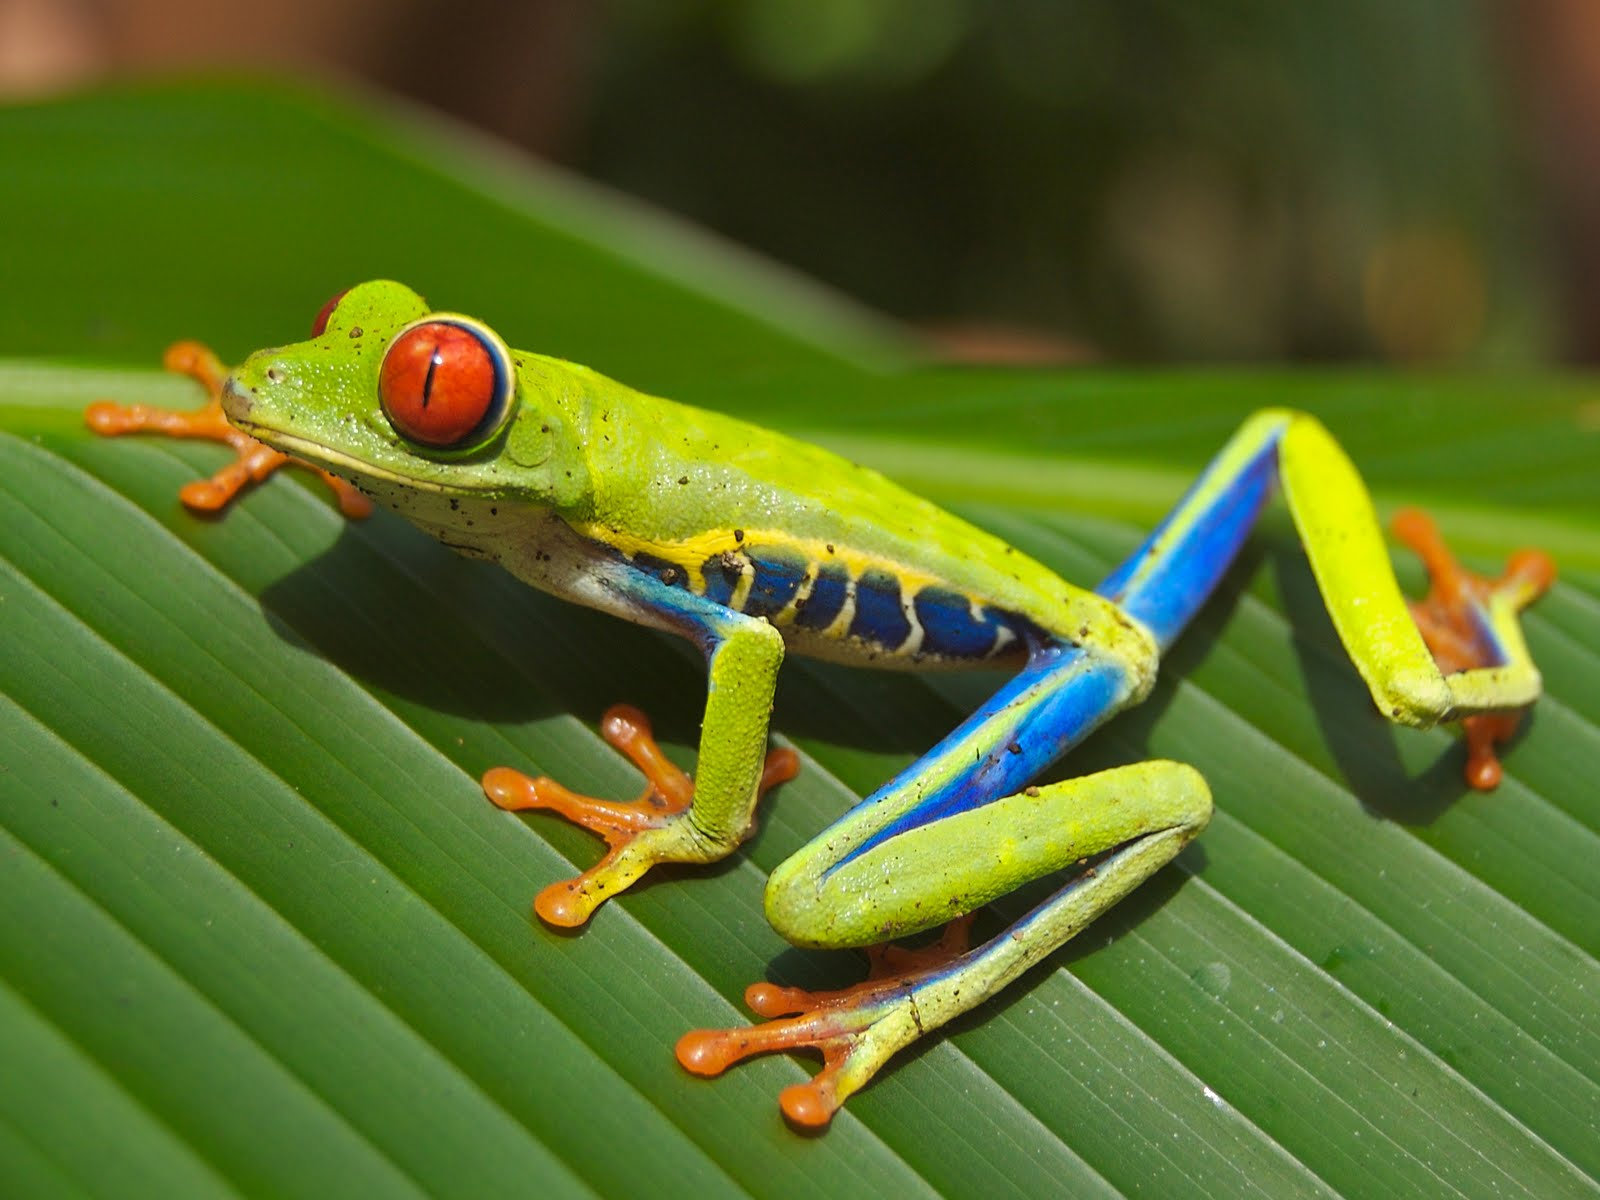
\includegraphics[scale=0.2]{frog.jpg}
		\caption{
			Step 1.
			A solution is delivered on coarse (4 elements) and fine grid (8 elements).
			Red line marks the coarse-grid solution, green line --- the fine-grid solution and black line --- the exact (analytic) solution.
		}
		\label{fig:h-adapt-two-grid-1}
	\end{subfigure}

	\begin{subfigure}[h]{1.0\textwidth}
		\centering
		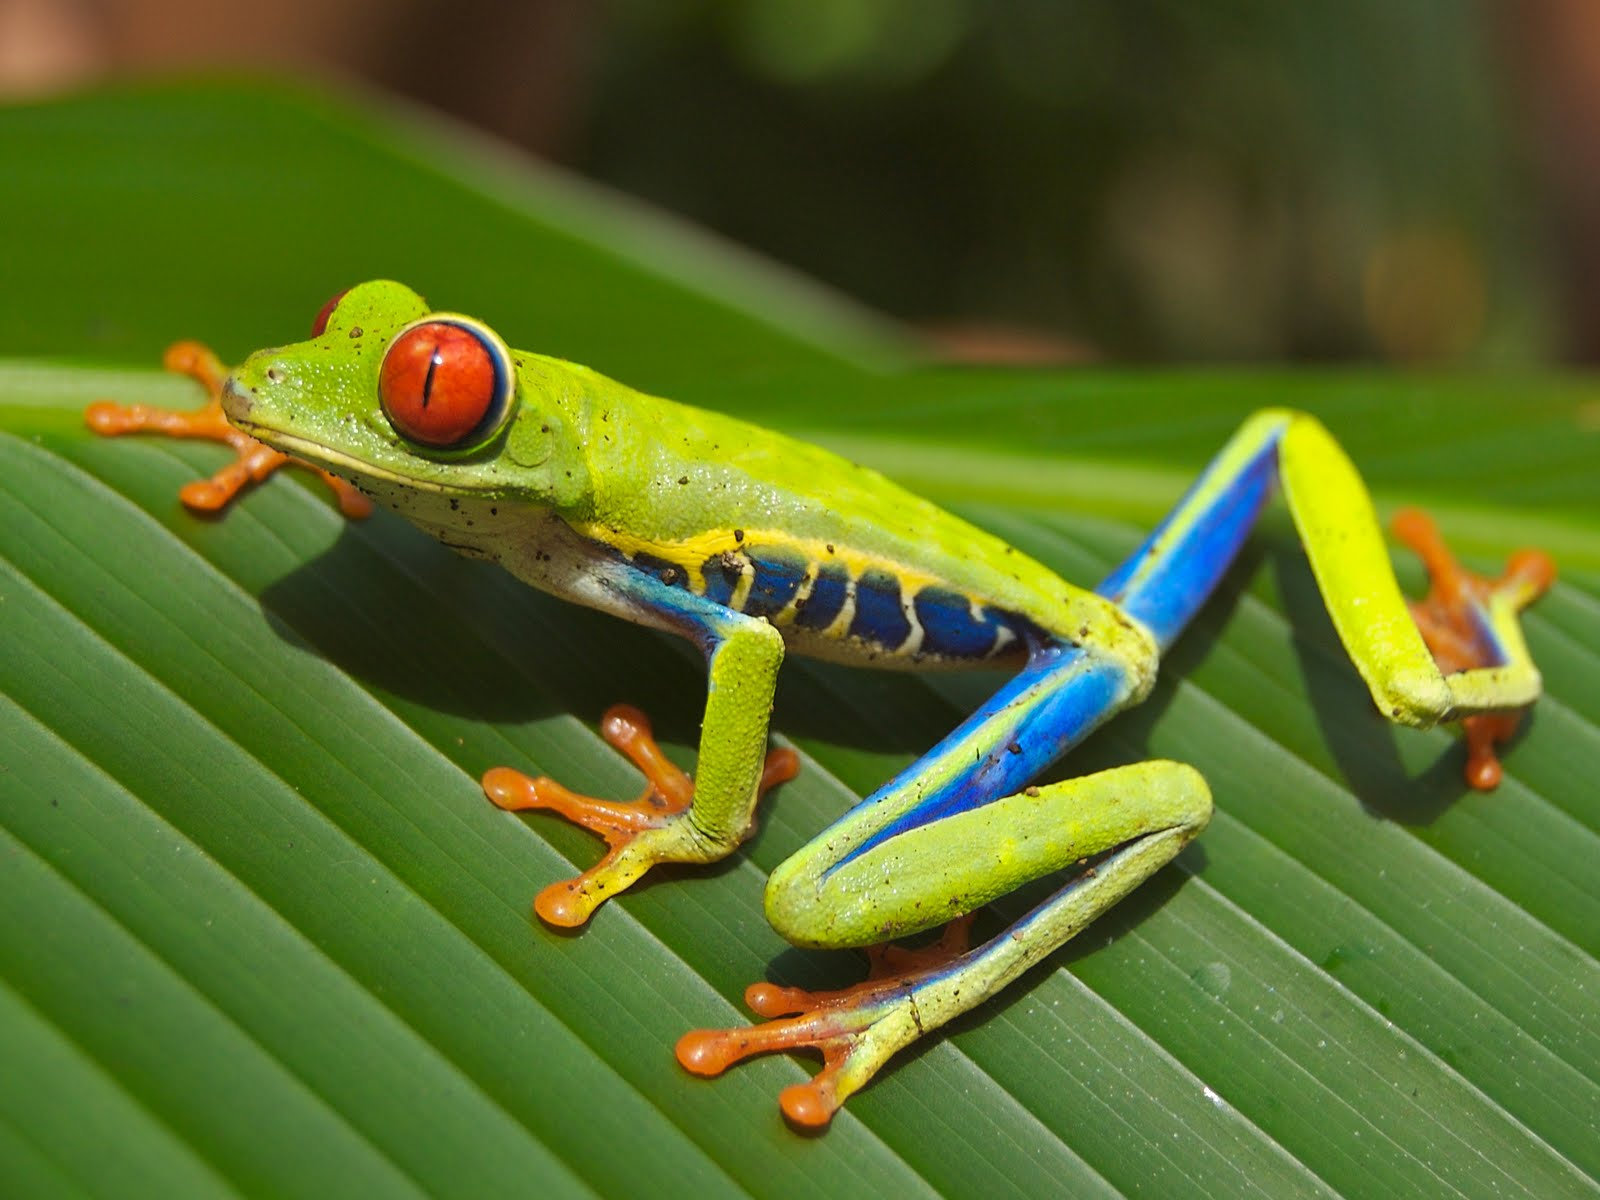
\includegraphics[scale=0.2]{frog.jpg}
		\caption{
			Step 2.
			Since the maximal error multiplied by $\tau$ (here set to 20\%) were lower than the error on any element,
			the algorithm halved all four elements after step 1.
		}
		\label{fig:h-adapt-two-grid-2}
	\end{subfigure}
\end{figure}


\begin{figure}[H]
	\ContinuedFloat % continue from previous page
	\caption[Double-grid h-adaptation strategy, steps 3-4]{} % for subcaption package to ensure proper numbering

	\begin{subfigure}[h]{1.0\textwidth}
		\centering
		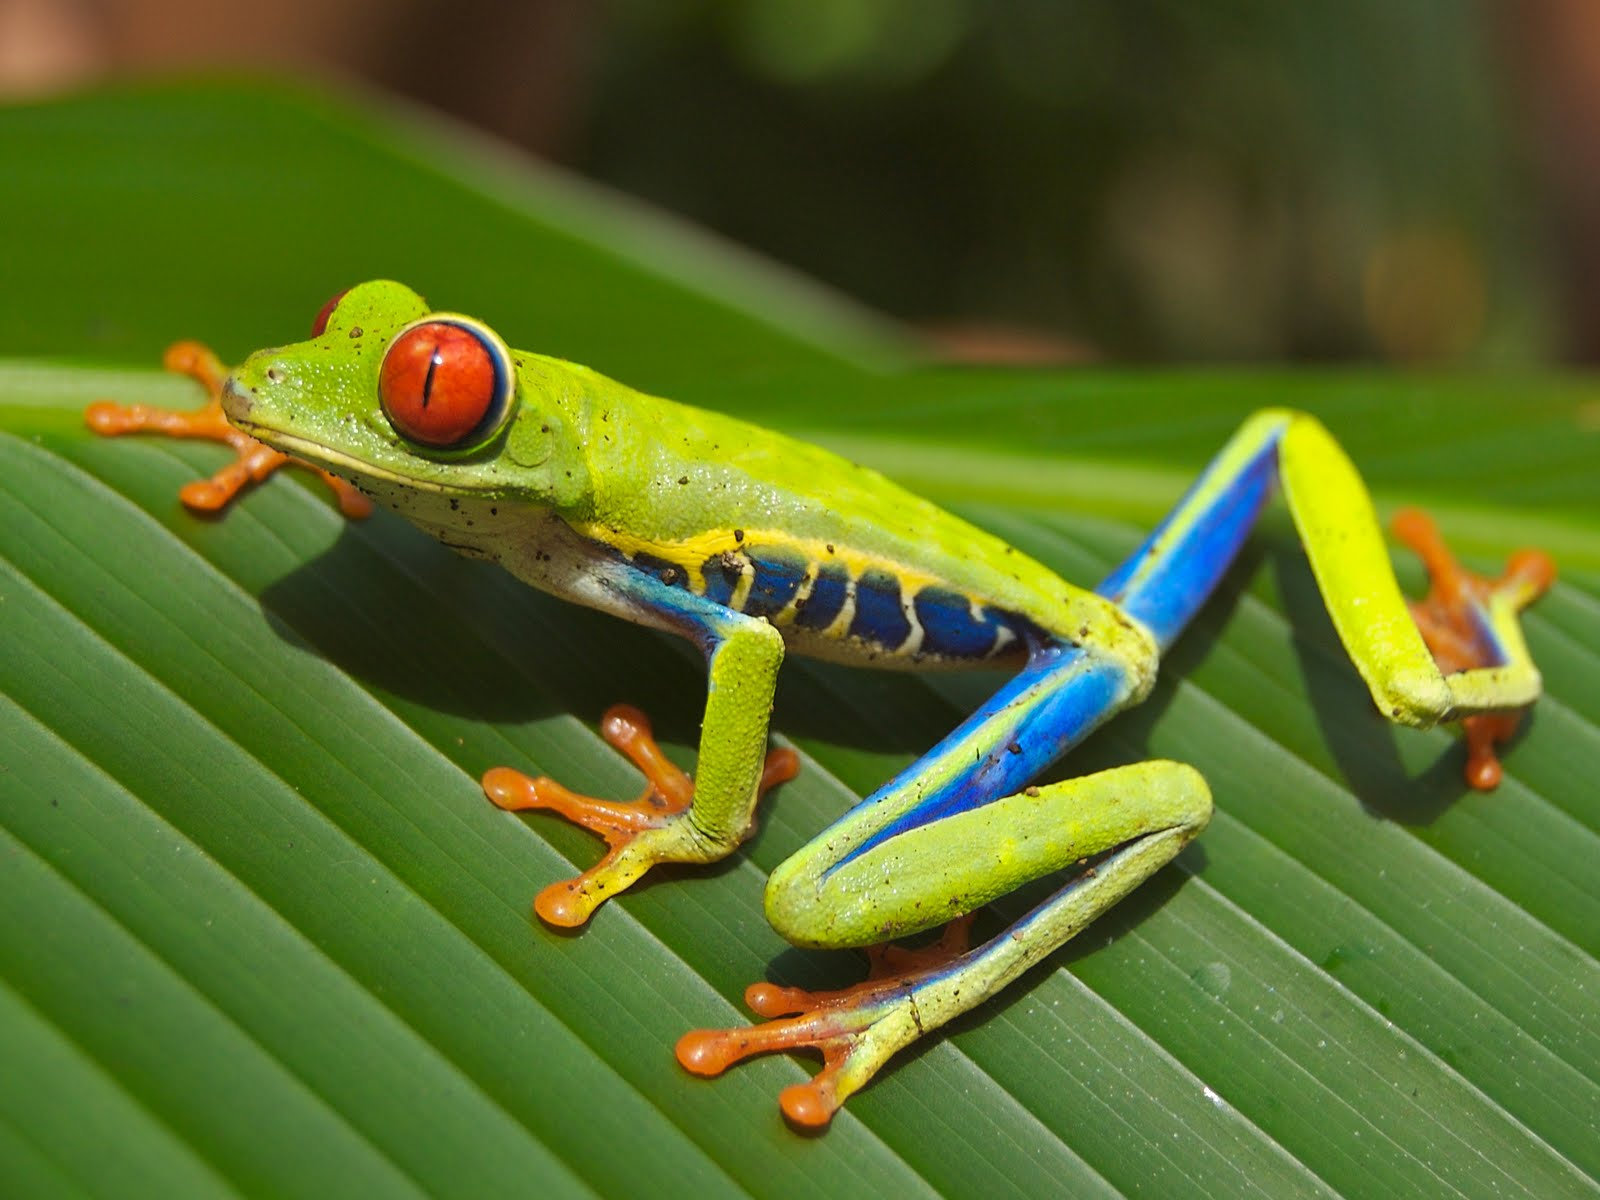
\includegraphics[scale=0.2]{frog.jpg}
		\caption{
			Step 3.
			The extreme left and right elements did not get refined after the step 2.
		}
		\label{fig:h-adapt-two-grid-3}
	\end{subfigure}

	\begin{subfigure}[h]{1.0\textwidth}
		\centering
		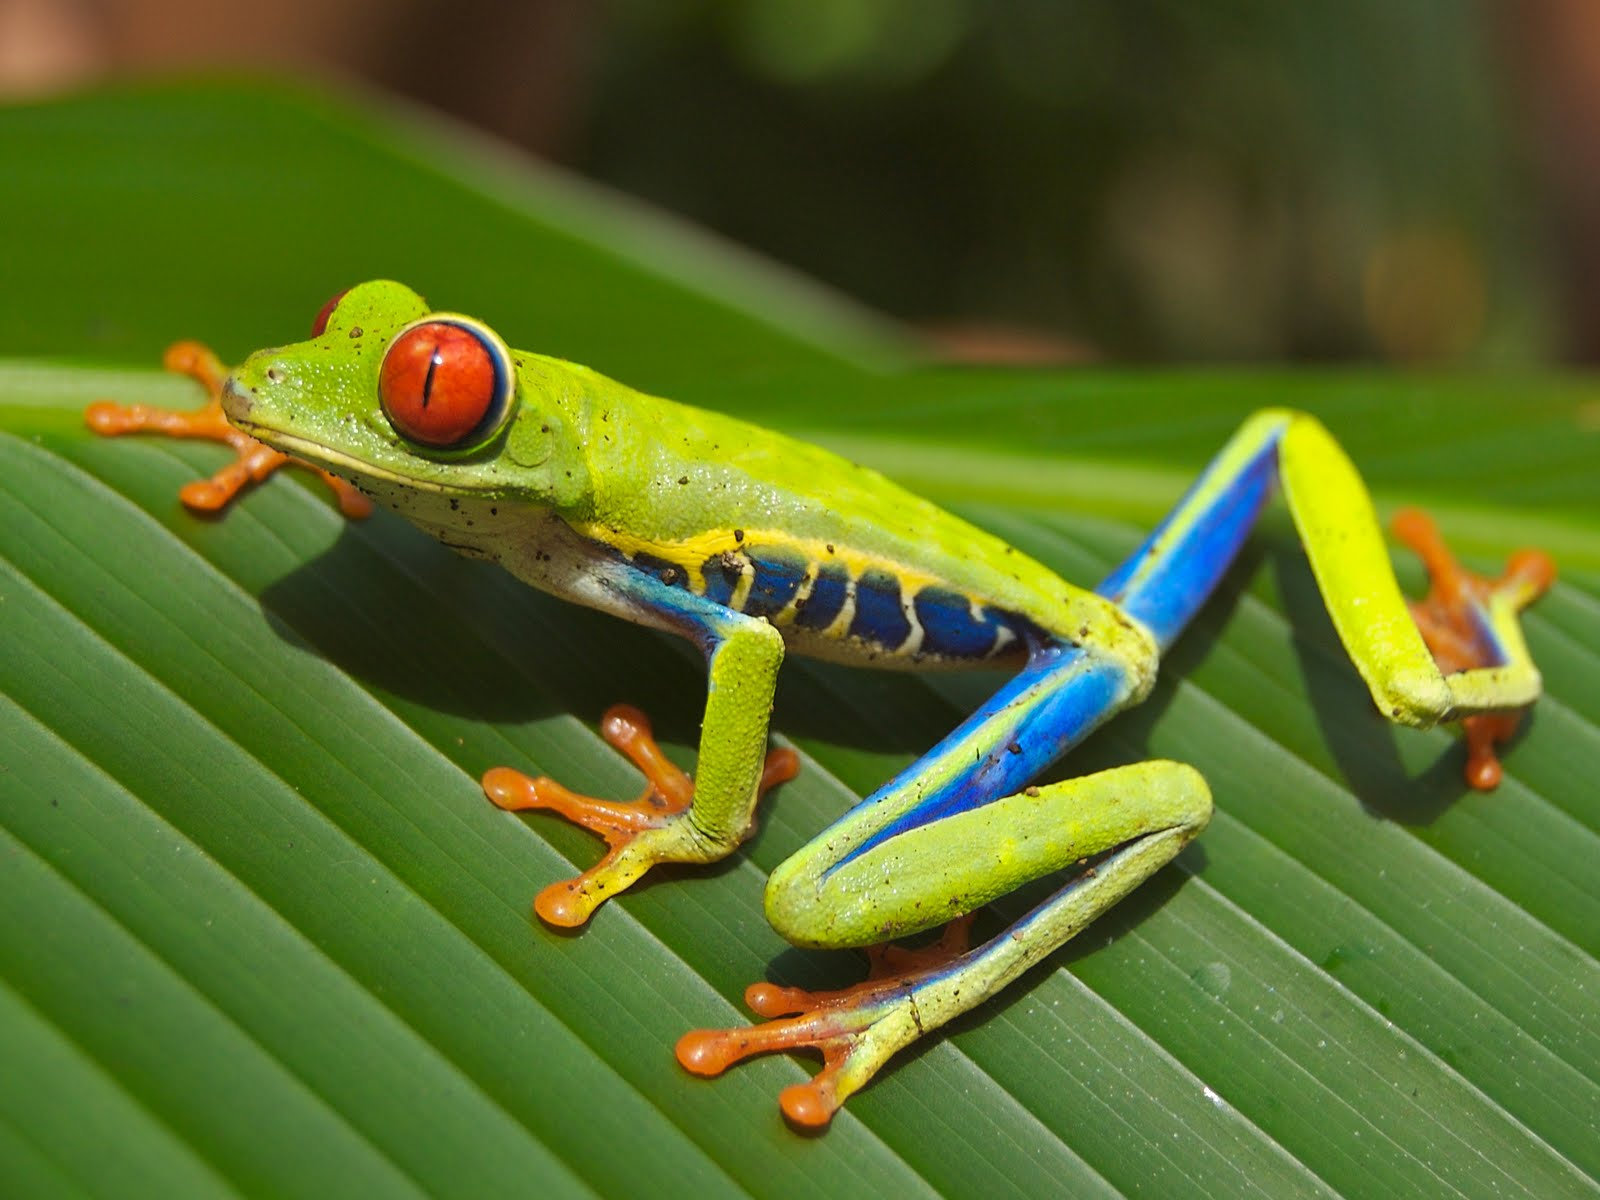
\includegraphics[scale=0.2]{frog.jpg}
		\caption{
			Step 4
		}
		\label{fig:h-adapt-two-grid-4}
	\end{subfigure}
\end{figure}




\chapter{Project documentation} \label{chap:docs}

\newcommand{\uml}[2] {
	\begin{figure}[H]
		\centering
		\caption{#1}
		\begin{mpost}[mpsettings=input metauml;]
			#2
		\end{mpost}
	\end{figure}
}

\bt

\section{Some clever stuff} \label{sec:cuda}

\bt

\section{API components overview} \label{sec:api-overview}

Nice UML no. 1...

\uml{IsogeometricFEM class} {
	Class.C("IsogeometricFEM") ()
		("+ apply(pde: PDE, bcs: BoundaryConditions,
			base: BsplineBase, solver: Solver, femConfig: FEMConfig)");
	drawObject(C);
}

Nice UML no. 2...

\uml{HAdaptiveIsogeometricFEM interface} {
	Interface.I("HAdaptiveIsogeometricFEM")
		("+ apply(pde: PDE, bcs: BoundaryConditions,
			adaptationThreshold: Double, solver: Solver, femConfig: FEMConfig)");
	classStereotypes.I("<<interface>>");
	drawObject(I);
}


\section{Detailed API specification and class diagrams} \label{sec:api-detail}

And another large UML...

\uml{The overall class diagram} {
	Class.IsogeometricFEM("IsogeometricFEM")
		() ("+ apply(...)");

	Class.PDE("PDE")
		("+ lhsCoefs: Function[1..*]", "+ rhs: Function") ();
	IsogeometricFEM.n = PDE.s + (60, -60);

	Class.BoundaryConditions("BoundaryConditions")
		("+ left: Double", "+ right: Double",
		 "+ leftType: BoundaryType", "+ rightType: BoundaryType") ();
	IsogeometricFEM.s = BoundaryConditions.n + (60, 60);

	Interface.Base("Base")
		("+ count(): Int",
		 "+ eval(...): Double",
		 "+ getSupport(no: Int): Range");
	classStereotypes.Base("<<interface>>");
	IsogeometricFEM.w = BsplineBase.e + (-150, 0);

	AbstractClass.GriddedBase("GriddedBase") ()
		("+ getGrid(): PointSequence",
		 "+ getGridSpan(index: Int): IntRange",
		 "+ getSupport(no: Int): Range");
	Base.n = GriddedBase.s + (-80, -60);

	Class.BsplineBase("BsplineBase") ()
		("+ getGrid(): PointSequence",
		 "+ getGridSpan(index: Int): IntRange",
		 "+ getSupport(no: Int): Range");
	Base.n = BsplineBase.s + (80, -60);

	Interface.Solver("Solver")
		("+ apply(...)");
	classStereotypes.Solver("<<interface>>");
	IsogeometricFEM.s = Solver.n + (-60, 60);

	Class.GaussSolver("GaussSolver")
		() ("+ apply(...)");
	Solver.e = GaussSolver.w + (-60, 0);

	Class.MultifrontalSolver("MultifrontalSolver")
		() ("+ apply(...)");
	Solver.s = MultifrontalSolver.n + (0, 60);


	drawObjects(
		IsogeometricFEM,
		PDE, BoundaryConditions,
		Base, GriddedBase, BsplineBase,
		Solver, GaussSolver, MultifrontalSolver
	);

	link(dependency)(IsogeometricFEM.n -- PDE.s);
	link(dependency)(IsogeometricFEM.n -- BsplineBase.s);
	link(dependency)(IsogeometricFEM.s -- BoundaryConditions.n);
	link(dependency)(IsogeometricFEM.s -- Solver.n);
	link(realization)(GriddedBase.s -- Base.n);
	link(realization)(BsplineBase.s -- Base.n);
	link(realization)(GaussSolver.w -- Solver.e);
	link(realization)(MultifrontalSolver.n -- Solver.s);
}



\chapter{Evaluation of the results} \label{chap:evaluation}

\bt

\section{e.g. Convergence analysis} \label{sec:convergence}

\bt

\section{e.g. Complexity analysis} \label{sec:complexity}

\bt

\section{e.g. Flood simulation results} \label{sec:flood-results}

\bt


\chapter{Conclusions and future works} \label{chap:conclusions}

\section{Achieved goals and observations}

\bt 

\section{Areas for development}

\bt


%%%%%%%%%%%%%%%%%%%%%%%%%%%%%%%%%%%%%
%%%%%%%%%%%%%%%%%%%%%%%%%%%%%%%%%%%%%
% \appendix % Dodatek
%%%%%%%%%%%%%%%%%%%%%%%%%%%%%%%%%%%%%
% Rozdziały dodatku
% \include{tex/example}
%%%%%%%%%%%%%%%%%%%%%%%%%%%%%%%%%%%%%
%%%%%%%%%%%%%%%%%%%%%%%%%%%%%%%%%%%%%
% \backmatter % Część końcowa
%%%%%%%%%%%%%%%%%%%%%%%%%%%%%%%%%%%%%
% Rozdziały części końcowej
% \include{tex/notes}
%%%%%%%%%%%%%%%%%%%%%%%%%%%%%%%%%%%%%
%%%%%%%%%%%%%%%%%%%%%%%%%%%%%%%%%%%%%
% UWAGA: Jeżeli będziesz tworzyć spis literatury ręcznie, tj. za pomocą otoczenia 
%  'thebibliography', to pamiętaj — powinien zawierać tylko te publikacje, 
%  do których odwołujesz się w pracy. 

% \nocite{*} % forces bibtex to include all citations, whether or not they were referred to in the paper

\printbibliography  % Wyświetl spis literatury
%%%%%%%%%%%%%%%%%%%%%%%%%%%%%%%%%%%%%
%%%%%%%%%%%%%%%%%%%%%%%%%%%%%%%%%%%%%
\end{document}